\chapter{The Brain}
Amongst the algorithms for choosing the moves in turn-based games, we chose the \textit{alpha-beta pruning} algorithm.
It is a well known algorithm for turn based games, and can be thinked of as an evolution of the basic minimax algorithm, in fact it aims to reduce the number of nodes that are evaluated during the search.

We will discuss the plain minimax algorithm, then the alpha-beta pruning one, and finally the way we used it in our specific case.

\section{Minimax} \label{sec:minimax}
\textit{Minimax} is an algorithm for making decisions.
The hipothesis is that of a 2 player zero-sum game, where the outcome goes from -V to V.

One of the player tries to maximize the outcome, while the other tries to minimize it.
For readability sake, we will refer to the two players as to \textbf{Max} and \textbf{Min}.

\textbf{Max} and \textbf{Min} alternate in choosing a move, so each turn consists into two choices, each of which is called a ``ply''.
At each level of the search, the active player watches the outcome associated with each of the options he has, and chooses the one that maximizes his result.
Since the outcome for each of the options depends on the next choice of the other player, the actual choice also minimizes the opponent's result.
This is why the name ``minimax''.\\

\begin{figure}[htbp]
  \centering
    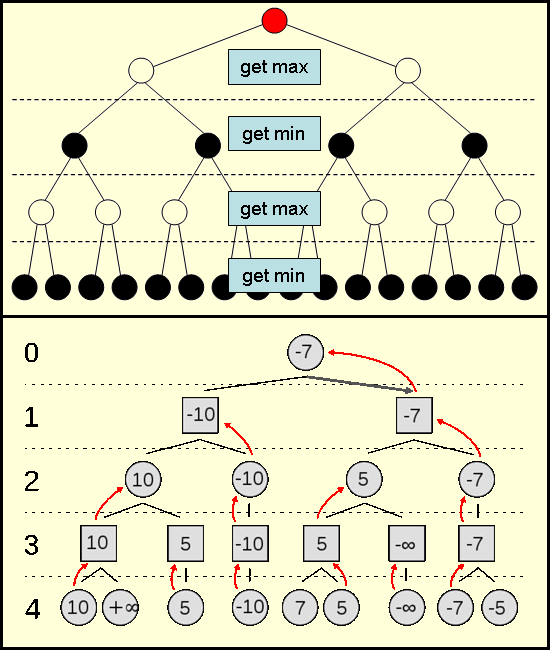
\includegraphics[width=0.5\textwidth]{images/minimax.png}
  \caption{Minimax choosing schema and a simple case example.}
\end{figure}

Of course, when the depth of the tree becomes too high to compute the actual outcome of a choice, we need to use some heuristics. Moreover, this algorithm assumes that the opponent plays with a ``perfect'' strategy, that is reasonable in normal turn-based games, but has some interesting effects when players choose more than a move each time (see chapter \ref{cap:results} for more on this).

\section{Alpha-Beta pruning}
As seen in section \ref{sec:minimax}, the \textit{minimax} algorithm expands the tree up to a certain level, evaluating all the leaf nodes and backpropagating informations.
While descending in new branches, it doesn't take into account the previously computed heuristic values.
The \textit{alpha-beta pruning} algorithm tries to reduce the number of explored nodes, pruning branches when they are doomed to not be chosen.

Basically, when the algorithm explores a child node, keeps in memory the value of the best alternative's value for the \textbf{Max} and \textbf{Min} players (respectively alpha and beta), taking into account their turns succession.
If the explored child's value turns out to be too good for the active player (the player associated with that search level), that is it is better than the value that the opponent can force the active player to obtain making another decision in a preceding level, the remaining children won't be explored.\\
\\
The pseudo-code will clarify:\\
{\footnotesize
\lstset{language=C}
\begin{lstlisting}
  function alphabeta(node, level, search_depth, alpha, beta,
                     				maximizing)
  {
    if level == search_depth	// this is a leaf node
    	return the heuristic value of the node
    
    if maximizing		// MAX player
    	for each child of node
        	alpha = max(alpha, alphabeta(child, level+1,
                			search_depth, alpha,
                        		beta, !maximizing)
                           )
                if beta <= alpha
                	break	// Beta cut-off
        return alpha
        
    else			// MIN player
    	for each child of node
        	beta = min(alpha, alphabeta(child, level+1,
                			search_depth, alpha,
                        		beta, !maximizing)
                           )
                if beta <= alpha
                	break	// Alpha cut-off
        return beta
  }
  
  -- first call:
  alphabeta(root, 0, search_depth, -infinite, +infinite, true)
\end{lstlisting}
}

\begin{figure}[htbp]
  \centering
    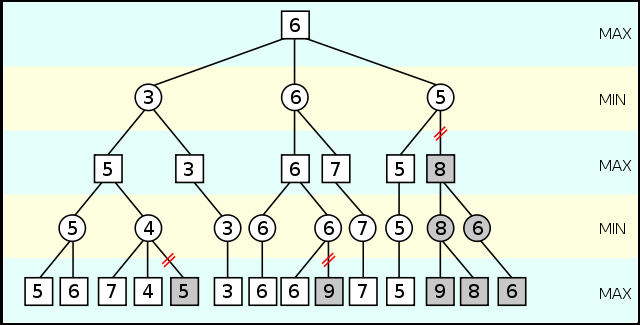
\includegraphics[width=0.5\textwidth]{images/alphabeta_pruning.png}
  \caption{Alpha-Beta Pruning use example. Darker nodes are not evaluated at all.}
  \label{fig:alphabeta_example}
\end{figure}

In figure \ref{fig:alphabeta_example} you can see a simple application of the alphabeta pruning algorithm. Notice that the algorithm, in some cases, prunes big portions of the tree. In the example given it may be a little advantage, but when the depth search and the branching factor grow this may lead to a huge resources saving.


\section{Adapting Alpha-Beta pruning to WOW}
There are several adaptations that we had to do in order to use this algorithm in our game.
We developed the algorithm taking into account the possible future advancements of the game, so we didn't stick to the \textit{2 cards} choice, but rather consider \textit{sequences} of cards.
Obviously, the cards set is also modifiable, and some moves may prevent the choice of other moves in sequence.

The algorithm takes into account all of these aspects, even if at the very moment they are not used in the game.\\

Since the heuristic function returns a discrete value, It is quite likely that two good sequences have the same result. In a sequential turn-based game\footnote{A game where a player moves after he has seen the opponent's move} either of the choices would be ok, so we could simply keep going with the first we found.
In a simultaneous turn-based game\footnote{In opposition with the sequential game, at each turn the players choose their moves simultaneously, without knowing the opponent's choice} like this, varying the strategy could help winning the game, because the opponent can't predict which will be the choice.

For this reason, we introduced a code block that, in the case that the computed heuristic of the newly analyzed sequence is the same value stored in alpha(if maximizing) or beta(if minimizing), there is a chance that the stored sequence is overwritten by the new one.
\vspace{2cm}


Pseudo-code of the algorithm:
{\footnotesize
  \lstset{language=C}
  \begin{lstlisting}
    global variables:
    	SEARCH_DEPTH		// levels to analyze
        MOVES_CHANGE		// chance to choose the new
        			// sequence when its heuristic
                                // equals the currently chosen
                                // sequence one
        CHOICES_PER_TURN	// how many moves must be chosen
    
    // each level of the search is a ply, so the search_depth
    // must be at least 2 times CHOICES_PER_TURN.
    
    
    algorithm:
    alphabeta(depth,maximizing,alpha,beta, actual_sequence, &choice)
      // 'choice' is side-effected to back-propagate informations.
      // it is the chosen sequence from the current node, the
      // parent of the current node could still discard it.
    { 
      if depth == SEARCH_DEPTH	// leaf node
      	choice = actual_sequence
        return the heuristic value of this sequence
      
      improved = false	// will be set to true if some better
      			// solution is found
      
      if maximizing	// MAX player
      	if the plane is dead
        	return a very low value
        if the plane can`t move remaining inside the field
        	return -infinity	// death is preferred
                			// over suicide
        
        child_seq = new empty sequence
        
        for each possible move
        	queue this move to actual_sequence
                update status	// move the planes
                child_heur = alphabeta(depth+1, !maximizing, alpha,
					beta, actual_sequence,
                                        child_seq)
                restore status
        	
                // now analyze the child
                up_seq = false	// tells whether child_seq should
				// become the new (locally)
                                // preferred sequence
                if alpha < child_heur
                	up_seq = true;
                if alpha == child_heur
                	put up_seq to true with
                        MOVES_CHANGE% probability
                        
                if up_seq
                	improved = true
                	alpha = child_heur
                	choice = child_seq
                
                if beta <= alpha
                	break	// beta cut-off (MIN player can do
				// better with different choices,
				// so we can avoid further searching)
      else		// MIN player
      	if the plane is dead
        	return a very high value (bad for MIN player)
        if the plane can`t move remaining inside the field
        	return +infinity	// death is preferred
                			// over suicide
        
        child_seq = new empty sequence
        
        for each possible move
        	queue this move to actual_sequence
                update status	// move the planes and inflict damages
                child_heur = alphabeta(depth+1, !maximizing, alpha,
					beta, actual_sequence,
                                        child_seq)
                restore status
        	
                // now analyze the child
                up_seq = false	// tells whether child_seq should
				// become the new (locally)
                                // preferred sequence
                if beta > child_heur
                	up_seq = true;
                if beta == child_heur
                	put up_seq to true with
                        MOVES_CHANGE% probability
                        
                if up_seq
                	improved = true
                	beta = child_heur
                	choice = child_seq
                
                if beta <= alpha
                	break	// alpha cut-off (MAX player can do
				// better with different choices,
				// so we can avoid further searching)
      if improved
      	return:	alpha if maximizing
        	beta if minimizing
      else
      	return:	-infinity if maximizing
        	+infinity if minimizing
    }
  \end{lstlisting}
}

There are other minor adjustments needed, one of all is due to the fact that, when the Human player manages to place itself in an advantage position, the AI may fail to find a sequence that doesn't cause its plane to die. This is even more likely with greater values of the search\_depth. What we actually need is only the first two moves, but the AI may look much further, and decide that, in 10 moves, it is doomed to lose, so it would throw away the whole sequence.
To avoid the plane to suicide itself, we added an ``emergency'' behaviour to be used in such cases, which will simply move the plane in order to remain inside the field. This also introduces unpredictable moves in the game.
